% Informe IEEE — FitoDiag-PY
% Compilar: pdflatex main && bibtex main && pdflatex main && pdflatex main
% Las cifras salen de tables/*.tex y tables/macros.tex, que genera scripts/compare_runs.py.
% Todo lo que esté en ROJO falta completar (\pend). Para la versión final, verificar que no quede rojo.
\documentclass[conference]{IEEEtran}
\usepackage[utf8]{inputenc}
\usepackage[T1]{fontenc}
\usepackage[spanish,es-tabla,es-nodecimaldot]{babel}
\usepackage{cite}
\usepackage{amsmath}
\usepackage{graphicx}
\usepackage{xcolor}
\usepackage{xurl}
\usepackage[hidelinks]{hyperref}

\newcommand{\pend}[1]{\textcolor{red}{#1}}
% Generado por scripts/compare_runs.py. No editar a mano.
\newcommand{\effAcc}{81.5}
\newcommand{\effFone}{80.4}
\newcommand{\effTop}{97.2}
\newcommand{\effMs}{53}
\newcommand{\effMsp}{75}
\newcommand{\effParams}{4.0}
\newcommand{\effMb}{16}
\newcommand{\effWrong}{0.0}
\newcommand{\effSoja}{72.8}
\newcommand{\effMandioca}{77.1}
\newcommand{\effSesamo}{97.0}
\newcommand{\effMin}{29}
\newcommand{\effWorstClass}{So-septo}
\newcommand{\effWorstFone}{56.8}
\newcommand{\resAcc}{81.5}
\newcommand{\resFone}{81.1}
\newcommand{\resTop}{97.3}
\newcommand{\resMs}{132}
\newcommand{\resMsp}{159}
\newcommand{\resParams}{23.5}
\newcommand{\resMb}{94}
\newcommand{\resWrong}{0.0}
\newcommand{\resSoja}{75.7}
\newcommand{\resMandioca}{75.5}
\newcommand{\resSesamo}{98.1}
\newcommand{\resMin}{30}
\newcommand{\resWorstClass}{So-frog}
\newcommand{\resWorstFone}{51.9}
\newcommand{\baseAcc}{80.4}
\newcommand{\baseFone}{78.7}
\newcommand{\baseTop}{94.8}
\newcommand{\baseMs}{58}
\newcommand{\baseMsp}{74}
\newcommand{\baseParams}{4.0}
\newcommand{\baseMb}{16}
\newcommand{\baseWrong}{0.1}
\newcommand{\baseSoja}{72.5}
\newcommand{\baseMandioca}{75.0}
\newcommand{\baseSesamo}{97.4}
\newcommand{\baseMin}{17}
\newcommand{\baseWorstClass}{So-frog}
\newcommand{\baseWorstFone}{47.4}
\newcommand{\dsRaw}{27719}
\newcommand{\dsKept}{13396}
\newcommand{\dsTrain}{9378}
\newcommand{\dsVal}{2009}
\newcommand{\dsTest}{2009}
\newcommand{\dsDup}{13}


\begin{document}

\title{FitoDiag-PY: Diagn\'ostico de Enfermedades Foliares en Soja, Mandioca y S\'esamo mediante Transferencia de Aprendizaje}

\author{\IEEEauthorblockN{Palmira Ben\'itez y Sebasti\'an Villalba}
\IEEEauthorblockA{\pend{Carrera, Facultad, Universidad}\\
\pend{Ciudad, Paraguay}\\
\pend{correo1@ejemplo.com, correo2@ejemplo.com}}}

\maketitle

\begin{abstract}
Las enfermedades foliares causan p\'erdidas importantes en la soja, la mandioca y el s\'esamo, tres rubros clave de la agricultura paraguaya. Presentamos FitoDiag-PY, un sistema de extremo a extremo que clasifica 15 condiciones foliares de estos cultivos a partir de una fotograf\'ia tomada con un tel\'efono m\'ovil. Unificamos tres conjuntos de datos p\'ublicos (\dsKept{} im\'agenes tras la limpieza) y comparamos el ajuste fino de EfficientNet-B0 y ResNet50, con aumento de datos orientado a fotos de campo y muestreo ponderado contra el desbalance de clases. En el conjunto de prueba, EfficientNet-B0 alcanz\'o una exactitud de \effAcc\,\% y un F1 macro de \effFone\,\%, con \effMs~ms de inferencia en CPU; ResNet50 obtuvo un F1 macro de \resFone\,\% con seis veces m\'as par\'ametros. El modelo se expone mediante una API REST y una interfaz web, empaquetadas en contenedores Docker que se despliegan con un solo comando.
\end{abstract}

\begin{IEEEkeywords}
visi\'on por computadora, fitopatolog\'ia, transferencia de aprendizaje, EfficientNet, Paraguay.
\end{IEEEkeywords}

\section{Introducci\'on y contexto}

La soja es el principal producto de exportaci\'on de Paraguay: para la campa\~na 2025/26 se proyecta una producci\'on r\'ecord de 12,3 millones de toneladas \cite{lanacion2026soja}. Su enfermedad m\'as importante en el pa\'is es la roya asi\'atica (\textit{Phakopsora pachyrhizi}) \cite{enciso2021roya}, que puede reducir el rendimiento hasta en un 80\,\% si no se controla a tiempo; en enero de 2026 el SENAVE emiti\'o una alerta fitosanitaria por esta causa \cite{lanacion2026roya}. La mandioca ocupa entre 160\,000 y 170\,000 hect\'areas, con una producci\'on cercana a 2 millones de toneladas, y es central para la agricultura familiar \cite{ultimahora2026mandioca}. El s\'esamo es el principal rubro de renta de la agricultura familiar campesina \cite{lanacion2024sesamo}. En los tres casos, el diagn\'ostico depende de que un t\'ecnico recorra el lote, algo dif\'icil de lograr a tiempo para los peque\~nos productores. Un error o un retraso en el diagn\'ostico lleva a aplicaciones tard\'ias o innecesarias de agroqu\'imicos.

\textit{Estado del arte.} Mohanty \textit{et al.} \cite{mohanty2016} alcanzaron 99,35\,\% de exactitud sobre PlantVillage, im\'agenes de hojas sobre fondo uniforme, pero la exactitud cay\'o a 31,4\,\% con im\'agenes de otras fuentes. Ferentinos \cite{ferentinos2018} report\'o resultados similares y la misma limitaci\'on. Por eso los trabajos recientes usan fotos de campo: el desaf\'io iCassava \cite{mwebaze2019icassava} y su sucesor en Kaggle \cite{kaggle2020cassava} para mandioca, y conjuntos tomados con smartphone para soja \cite{shinde2024soya} y s\'esamo \cite{sesame2025dataset}. Entre las arquitecturas, ResNet \cite{he2016resnet} introdujo las conexiones residuales y EfficientNet \cite{tan2019efficientnet} escala de forma conjunta profundidad, ancho y resoluci\'on con muchos menos par\'ametros. Para el desbalance, el sobremuestreo es la estrategia m\'as efectiva en redes convolucionales \cite{buda2018imbalance}, y el aumento de datos reduce el sobreajuste cuando hay pocas im\'agenes \cite{shorten2019augmentation}.

\textit{Contribuci\'on.} (i) Un conjunto de datos unificado y documentado para tres cultivos relevantes en Paraguay; (ii) una comparaci\'on controlada de dos arquitecturas, con una ablaci\'on de las t\'ecnicas contra el desbalance; y (iii) un sistema desplegable con un solo comando, apto para una demostraci\'on con un celular.

\section{Metodolog\'ia y arquitectura del sistema}

\subsection{Datos y preprocesamiento}
Se combinaron tres fuentes p\'ublicas de fotos de campo: MH-SoyaHealthVision para soja (6 clases, India) \cite{shinde2024soya}, Cassava Leaf Disease Classification para mandioca (5 clases, Uganda) \cite{kaggle2020cassava} y Sesame Leaf Disease para s\'esamo (4 clases, Bangladesh) \cite{sesame2025dataset}. Cada imagen se asign\'o a una clase \texttt{cultivo\_\_enfermedad}. El preprocesamiento (i) descart\'o archivos ilegibles y duplicados exactos por hash MD5 (\dsDup{} duplicados); (ii) us\'o solo las im\'agenes originales del s\'esamo, pues el dataset incluye copias aumentadas que filtrar\'ian informaci\'on entre particiones; (iii) limit\'o cada clase a 1\,500 im\'agenes, ya que el mosaico de la mandioca concentra la mayor\'ia de su conjunto; (iv) redimension\'o el lado mayor a 512 px; y (v) dividi\'o de forma estratificada en 70/15/15\,\% con semilla fija. La Tabla~\ref{tab:dataset} resume el resultado.

\begin{table}[t]
\caption{Conjunto de datos unificado (im\'agenes por partici\'on)}
\label{tab:dataset}
\centering\small
\begin{tabular}{lrrrr}
\hline
Cultivo & Clases & Train & Val & Test \\
\hline
Soja & 6 & 1939 & 415 & 415 \\
Mandioca & 5 & 4961 & 1063 & 1063 \\
S\'esamo & 4 & 2478 & 531 & 531 \\
\hline
Total & 15 & 9378 & 2009 & 2009 \\
\hline
\end{tabular}

\end{table}

\subsection{Modelos y entrenamiento}
Se compararon EfficientNet-B0 \cite{tan2019efficientnet} y ResNet50 \cite{he2016resnet}, ambos preentrenados en ImageNet (biblioteca timm \cite{wightman2019timm}), con la misma receta: entrada de $224\times224$, dos \'epocas entrenando solo la capa de clasificaci\'on y luego hasta 15 \'epocas de ajuste fino completo con AdamW (tasa $3\times10^{-4}$, decaimiento $10^{-4}$), programaci\'on coseno, \textit{label smoothing} de 0,1 y parada temprana sobre el F1 macro de validaci\'on (paciencia 5). Se entren\'o en una GPU T4 de Google Colab con precisi\'on mixta.

El aumento de datos simula fotos tomadas en el campo: recorte aleatorio (50--100\,\% del \'area), giros horizontales y verticales, rotaci\'on de $\pm25^{\circ}$, variaci\'on de brillo, contraste y saturaci\'on ($\pm40$\,\%), desenfoque gaussiano y borrado aleatorio de regiones (oclusiones). Contra el desbalance se us\'o un muestreador ponderado con probabilidad inversa a la frecuencia de cada clase \cite{buda2018imbalance}. Para medir el aporte de ambas t\'ecnicas se entren\'o una l\'inea base EfficientNet-B0 sin ellas.

\subsection{M\'etricas}
Por el desbalance, la m\'etrica principal es el F1 macro. Se reportan adem\'as la exactitud, la exactitud top-3, la tasa de cultivo equivocado (predicci\'on de un cultivo distinto al real) y la latencia en CPU con lote de una imagen y dos hilos (media de 50 ejecuciones tras 10 de calentamiento), que corresponde al contenedor de la API.

\subsection{API e interfaz}
La Fig.~\ref{fig:arq} muestra la arquitectura. La API en FastAPI expone \texttt{GET /health}, \texttt{GET /classes} y \texttt{POST /predict}. Este \'ultimo recibe la imagen, corrige la orientaci\'on EXIF del celular, aplica la misma transformaci\'on que la validaci\'on y devuelve la clase, la probabilidad, las tres clases m\'as probables, una sugerencia de manejo y el tiempo de inferencia. Si la probabilidad es menor a 0,5, la respuesta indica que el modelo no est\'a seguro y pide otra foto. La interfaz en Streamlit permite subir la foto o tomarla con la c\'amara desde el navegador del celular y solo se comunica con la API. Ambos servicios corren en contenedores Docker orquestados con \texttt{docker compose}; el modelo se monta como volumen de solo lectura.

\begin{figure}[t]
\centering
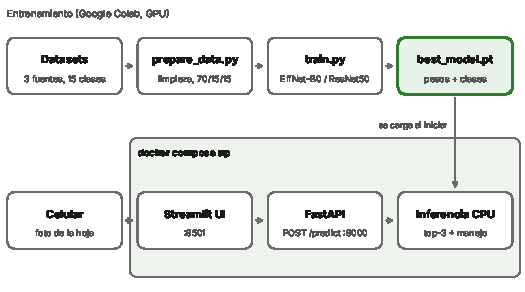
\includegraphics[width=\columnwidth]{figures/arquitectura.pdf}
\caption{Arquitectura: entrenamiento fuera de l\'inea y servicio en contenedores.}
\label{fig:arq}
\end{figure}

\section{Resultados y discusi\'on}

La Tabla~\ref{tab:results} resume el desempe\~no en el conjunto de prueba (\dsTest{} im\'agenes). EfficientNet-B0 obtuvo un F1 macro de \effFone\,\% y ResNet50, de \resFone\,\%. Ambos alcanzaron la misma exactitud (\effAcc\,\%) y la diferencia de F1 es menor a un punto, por lo que se consideran equivalentes; tampoco difieren en la exactitud top-3 (\effTop{} y \resTop\,\%). En latencia, EfficientNet-B0 tard\'o \effMs~ms por imagen en CPU frente a \resMs~ms de ResNet50, con 4,0 frente a 23,5 millones de par\'ametros. Por esa raz\'on se eligi\'o EfficientNet-B0 para la API.

\begin{table}[t]
\caption{Desempe\~no en el conjunto de prueba}
\label{tab:results}
\centering\small
\setlength{\tabcolsep}{4pt}
\begin{tabular}{lrrrrr}
\hline
Modelo & Params & Acc. & F1$_{macro}$ & Top-3 & CPU \\
 & (M) & (\%) & (\%) & (\%) & (ms) \\
\hline
EfficientNet-B0 & 4.0 & 81.5 & 80.4 & 97.2 & 53 \\
ResNet50 & 23.5 & 81.5 & \textbf{81.1} & 97.3 & 132 \\
EffNet-B0 base$^{\dagger}$ & 4.0 & 80.4 & 78.7 & 94.8 & 58 \\
\hline
\end{tabular}
\\[2pt]
\footnotesize $^{\dagger}$Sin aumento de datos ni muestreo ponderado.
\end{table}

La ablaci\'on mide el aporte de las t\'ecnicas contra el desbalance: sin aumento de datos ni muestreo ponderado, el F1 macro de EfficientNet-B0 fue \baseFone\,\%, frente a \effFone\,\% con ellas. La mejora se concentra en la sensibilidad: el \textit{recall} macro sube de 78,0 a 80,9\,\%, mientras la precisi\'on se mantiene (80,6 y 80,1\,\%). Sin balanceo, el modelo favorece a las clases mayoritarias y deja de reconocer las minoritarias. La Fig.~\ref{fig:curves} muestra la evoluci\'on del F1 macro de validaci\'on: las dos primeras \'epocas corresponden al entrenamiento de la capa de clasificaci\'on, y el salto posterior, al ajuste fino de toda la red. La l\'inea base alcanza una exactitud de entrenamiento de 100\,\% desde la octava \'epoca de ajuste fino sin mejorar en validaci\'on: memoriza el conjunto de entrenamiento. Con aumento de datos, la exactitud de entrenamiento se estabiliza en 92\,\%. ResNet50 obtuvo su mejor F1 en la \'ultima \'epoca, por lo que podr\'ia mejorar con un entrenamiento m\'as largo.

\begin{figure}[t]
\centering
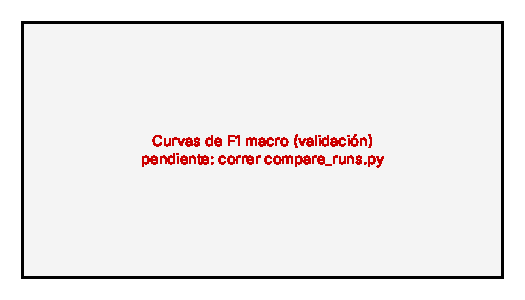
\includegraphics[width=\columnwidth]{figures/curves.pdf}
\caption{F1 macro de validaci\'on por \'epoca para las tres configuraciones.}
\label{fig:curves}
\end{figure}

Por cultivo (Tabla~\ref{tab:crop}), la exactitud de EfficientNet-B0 fue \effSoja\,\% en soja, \effMandioca\,\% en mandioca y \effSesamo\,\% en s\'esamo.

\begin{table}[t]
\caption{Exactitud por cultivo en prueba (\%)}
\label{tab:crop}
\centering\small
\begin{tabular}{lrrr}
\hline
Cultivo & EfficientNet-B0 & ResNet50 & Base$^{\dagger}$ \\
\hline
Soja & \effSoja & \resSoja & \baseSoja \\
Mandioca & \effMandioca & \resMandioca & \baseMandioca \\
S\'esamo & \effSesamo & \resSesamo & \baseSesamo \\
\hline
Cultivo equivocado & \effWrong & \resWrong & \baseWrong \\
\hline
\end{tabular}
\end{table}

 La clase con menor F1 fue \effWorstClass{} (\effWorstFone\,\%). La matriz de confusi\'on (Fig.~\ref{fig:cm}) muestra que la mayor\'ia de los errores ocurren dentro de un mismo cultivo: solo el \effWrong\,\% de las predicciones se equivoc\'o de cultivo. En soja, el 23\,\% de las hojas con mancha marr\'on se clasific\'o como roya, ambas con lesiones peque\~nas y oscuras; esta confusi\'on genera falsas alarmas, mientras que el caso inverso (14\,\% de la roya clasificada como mancha marr\'on) es m\'as grave, porque demora el control. En mandioca, la confusi\'on principal es entre hojas enfermas y sanas: el 14\,\% de la bacteriosis y el 11\,\% de la estr\'ia marr\'on se predijeron como sanas, lo que es coherente con s\'intomas tempranos poco visibles y con el ruido de etiquetado conocido de este conjunto \cite{mwebaze2019icassava}.

\begin{figure}[t]
\centering
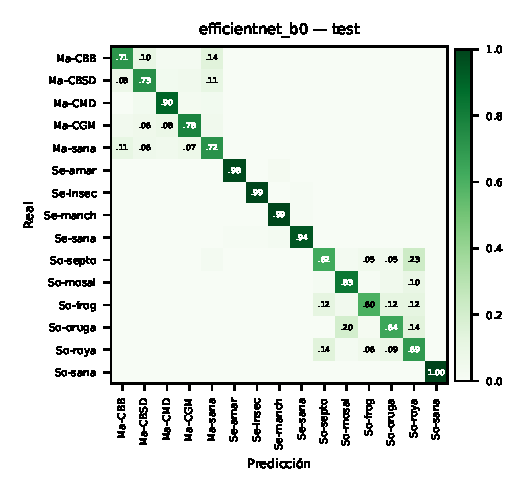
\includegraphics[width=0.85\columnwidth]{figures/confusion_matrix.pdf}
\caption{Matriz de confusi\'on normalizada por fila de EfficientNet-B0 en prueba. Ma: mandioca; Se: s\'esamo; So: soja.}
\label{fig:cm}
\end{figure}

Estas cifras miden el desempe\~no con im\'agenes de la misma distribuci\'on que el entrenamiento. Como mostraron Mohanty \textit{et al.} \cite{mohanty2016}, el desempe\~no cae con fotos de otras fuentes, y ninguna imagen del conjunto proviene de Paraguay. \pend{[Si probaron con fotos propias tomadas en Paraguay, reportar aqu\'i cu\'antas y cu\'antas acert\'o.]} El umbral de confianza mitiga el riesgo: ante una foto at\'ipica, el sistema pide otra imagen en lugar de dar un diagn\'ostico.

\section{Conclusiones y trabajo futuro}

FitoDiag-PY demuestra que un modelo liviano como EfficientNet-B0, ajustado sobre datos p\'ublicos de campo, puede diagnosticar enfermedades foliares de tres cultivos paraguayos en \effMs~ms por imagen sin GPU, dentro de un sistema que se despliega con un solo comando. Tres lecciones surgieron del proyecto. Primero, unificar los datos llev\'o m\'as trabajo que entrenar los modelos. Segundo, los conjuntos con im\'agenes aumentadas de f\'abrica pueden inflar las m\'etricas si no se separan antes de dividir. Tercero, con clases desbalanceadas la exactitud global oculta los errores en las clases minoritarias, por lo que conviene reportar el F1 macro.

Las limitaciones principales son la ausencia de im\'agenes paraguayas y dos enfermedades de la mandioca (mosaico y estr\'ia marr\'on) que no est\'an reportadas en Am\'erica, por lo que la API advierte al usuario si las detecta. Adem\'as, las fotos de mandioca suelen mostrar la planta entera y las de soja y s\'esamo una sola hoja, por lo que el modelo podr\'ia aprender el tipo de foto antes que el cultivo. Como trabajo futuro se propone (i) recolectar y etiquetar fotos en Paraguay junto con t\'ecnicos de campo; (ii) filtrar las clases seg\'un el cultivo indicado por el usuario; (iii) cuantizar el modelo para usarlo sin conexi\'on en el celular; (iv) agregar mapas de activaci\'on (Grad-CAM) para explicar cada diagn\'ostico; y (v) ofrecer la interfaz en guaran\'i.

\bibliographystyle{IEEEtran}
\bibliography{references}

\end{document}
